\section{Introduction to nonlinear Schwarz methods}

\begin{frame}{Motivation: linear vs nonlinear preconditioning}
	Discretized nonlinear partial differential equation: $F(u) = 0$
	\begin{columns}
		\begin{column}{0.5\textwidth}
			\vspace*{-4mm}
			\begin{block}{\normalsize Linear preconditioner}
				\begin{enumerate}
					\item Linearize:
					      \begin{equation*}
						      DF(u^k)\delta^{k+1} = F(u^k)
					      \end{equation*}
					\item Improve linear solver performance with Schwarz preconditioner:
					      \begin{equation*}
						      \mathcal{M}_{OS}^{-1}DF(u^k)\delta^{k+1} = \mathcal{M}_{OS}^{-1}F(u^k)
					      \end{equation*}
				\end{enumerate}
				\vspace*{4mm}
				Goal:
				\begin{itemize}
					\item $\kappa(\mathcal{M}_{OS}^{-1}DF(u^k)) \approx 1$
				\end{itemize}
			\end{block}
		\end{column}
		\begin{column}{0.5\textwidth}
			\vspace*{-4mm}
			\begin{block}{\normalsize Nonlinear preconditioner}
				\begin{enumerate}
					\item Reformulate the original nonlinear problem based on local nonlinear corrections
					      \begin{equation}
						      \mathcal{F}(u) = G(F(u)) = 0
					      \end{equation}
					\item Linearize $\mathcal{F}(u) = 0$ and solve iterativily
				\end{enumerate}
				Goal:
				\begin{itemize}
					\item $\mathcal{F}(u)$ more linear than $F(u)$
					\item $\mathcal{F}(u^*) = 0 \iff F(u^*) = 0$
				\end{itemize}
			\end{block}
		\end{column}
	\end{columns}
\end{frame}

\begin{frame}{Some References on Nonlinear Domain Decomposition Methods}
\tiny
\textbf{Nonlinear FETI-DP and Nonlinear BDDC:}\\
Klawonn, Lanser, Rheinbach (2012, 2013, 2014, 2015, 2016, 2018), Klawonn, Lanser, Rheinbach, Uran (2017, 2018), Klawonn Lanser, Uran (2021, 2023), \dots\\~\\

\textbf{Nonlinear Elimination:}\\
Hwang, Lin, Cai (2010); Cai, Li (2011); Wang, Su, Cai (2015); Hwang, Su, Cai (2016); Gong, Cai (2018); Luo, Shiu, Chen, Cai (2019); Gong, Cai (2019); Liu, Hwang, Luo, Cai, Keyes (2022), \dots\\~\\

\textbf{ASPIN:}\\
Cai, Keyes 2002; Cai, Keyes, Marcinkowski 2002; Hwang, Cai 2005, 2007; Groß, Krause (2010, 2013), \dots\\~\\

\textbf{MSPIN and Field-split methods:}\\
Keyes, Liu, (2015, 2016,2021); Liu, Wei, Keyes (2017); Kopanicáková, Kothari, Krause (2023), \dots\\~\\

\textbf{RASPEN:}\\
Dolean, Gander, Kherijii, Kwok, Masson (2016)\\~\\

\textbf{Nonlinear 2-Level Schwarz:}\\
Heinlein, Lanser (2020); Heinlein, Klawonn, Lanser (2022)\\~\\

\textbf{Nonlinear Neumann-Neumann:}\\ Bordeu, Boucard, Gosselet 2009\\~\\

\textbf{Nonlinear FETI-1:}\\
Pebrel, Rey, Gosselet 2008; Negrello, Gosselet, Rey (2021)\\~\\

\textbf{Other DD work reversing linearization and decomposition:}\\
Ganis, Juntunen, Pencheva, Wheeler, Yotov 2014; Ganis, Kumar, Pencheva, Wheeler, Yotov 2014
\end{frame}

\begin{frame}{One-level nonlinear Schwarz \footnote{\tiny Cai and Keyes 2002}}%: Nonlinearly preconditioned inexact Newton algorithms}}
	% \only<1-3>{
		Discretized nonlinear partial differential equation: F (u) = 0
	    \vspace*{-5mm}
	% }
	% \only<4->{
	%     \vspace*{-10mm}
	% }

	\begin{columns}
		\begin{column}{0.5\textwidth}
			\begin{block}<1->{\normalsize Nonlinear corrections $T_i(u): V\mapsto V_i$}
				\vspace*{-5mm}
				\begin{align*}
					 & R_iF(u-P_iT_i(u))  = 0, \quad i = 1,2,\dots N                \\
					 & \text{with}\quad R_i:V\mapsto V_i\text{,}\, P_i:V_i\mapsto V
				\end{align*}
			\end{block}
		\end{column}
		\begin{column}{0.5\textwidth}
			\begin{block}<2->{\normalsize Define an alternative nonlinear problem}
				\begin{equation*}
					\mathcal{F}_1(u) \coloneqq \sum_{i=1}^N\alert<4>{P_iT_i(u)} = 0
				\end{equation*}
			\end{block}
		\end{column}
	\end{columns}
	\begin{block}<3->{\normalsize Nonlinear Schwarz method results by solving $\mathcal{F}_1(u) = 0$ with Newton's method.\newline Setting $u_i = u-P_iT_i(u)$ the Jacobian can be formulated as:}
		\vspace*{-2mm}
		\begin{align*}
			D\mathcal{F}_1(u^k)  = \sum_{i = 1}^NP_iDT_i(u^k) = \sum_{i=1}^N\alert<4>{P_i(R_iDF(u_i^k)P_i)^{-1}R_iDF(u_i^k)}
		\end{align*}
	\end{block}
	\only<4>{%
		\tikz[overlay,remember picture]
		\node[fill=white,text=red] at ([xshift=0cm,yshift=-3cm]current page.center){\Large Parallel execution!};
	}
	% \only<4>{%
	% \begin{itemize}
	% 	\item For the one-level nonlinear Schwarz method the solutions of $F(u) = 0$ and $\mathcal{F}_1(u) = 0$ are equivalent
	% 	\item The global operators $DF(u_i)$ only need to be assembled locally
	% \end{itemize}
	% }
\end{frame}

\begin{frame}{Adding a second level}
	Build coarse space basis functions $\rightarrow$ $R_0$ and $P_0$ 
    \begin{block}{RGDSW coarse space \footnotemark{}}
		Define coarse basis $\Phi : V_0\mapsto V$
		\begin{enumerate}
			\setlength{\itemsep}{10pt}
			\item Build $\Phi_\Gamma$ as a partition of unity on the interface $\Gamma$
			\item $\Phi_I = -A_{II}^{-1}A_{I\Gamma}\Phi_\Gamma$ an energy minimizing extension into the interior
		\end{enumerate}
	\end{block}
	\only<2>{ % Compile twice for proper placement
		For example:
		\begin{columns}
			\begin{column}{0.39\textwidth}
				\vspace*{-6mm}
				\begin{figure}
					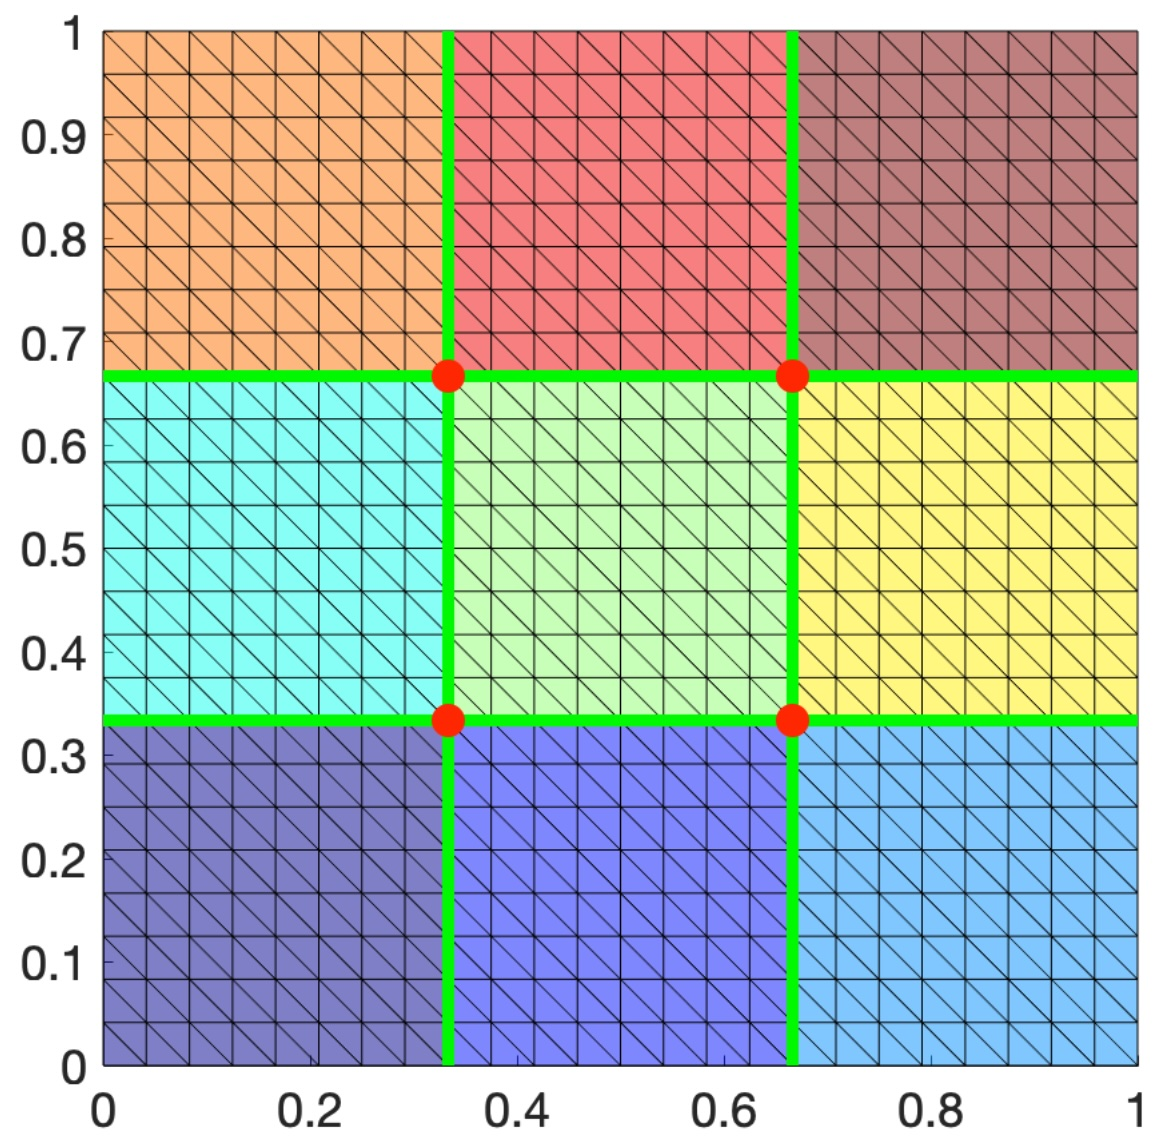
\includegraphics[width=0.45\textwidth]{images/decomposed_domain.jpg}
				\end{figure}
			\end{column}
            \hspace*{-20mm}
			\begin{column}{0.4\textwidth}
				\vspace*{-9mm}
				\begin{figure}
					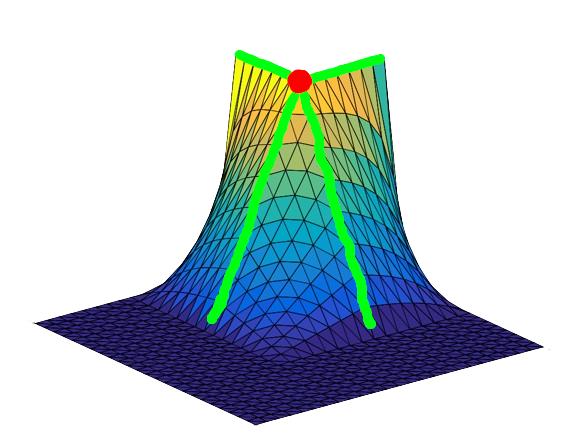
\includegraphics[width=0.65\textwidth]{images/r22.png}
				\end{figure}
			\end{column}
		\end{columns}
	}
	\only<3>{
		Summary:
		\begin{equation*}
			\Phi =
			\begin{pmatrix}
				\Phi_I \\  \Phi_\Gamma
			\end{pmatrix} =
			\begin{pmatrix}
				-A_{II}^{-1}A_{I\Gamma}\Phi_\Gamma \\ \Phi_\Gamma
			\end{pmatrix}
		\end{equation*}
		and
		\begin{equation*}
			P_0 \coloneqq \Phi\text{,}\quad R_0 \coloneqq \Phi^T
		\end{equation*}
	}
\footnotetext{\tiny Dohrmann, Widlund (2017)}
\end{frame}

\begin{frame}{Two-level additive nonlinear Schwarz \footnote{\tiny Heinlein, Lanser (2020)} \footnote{\tiny Heinlein, Lanser, Klawonn (2022)}}
	% \vspace*{-5mm}
	\begin{columns}
		\begin{column}{0.5\textwidth}
			\begin{block}{\normalsize Nonlinear corrections $T_i(u)$}
				\vspace*{-1mm}
				\begin{align*}
					 & R_iF(u-P_iT_i(u))  = 0, \quad i = \alert{0},1,2,\dots N      \\
					 & \text{with}\quad R_i:V\mapsto V_i\text{,}\, P_i:V_i\mapsto V
				\end{align*}
			\end{block}
		\end{column}
		\begin{column}{0.5\textwidth}
			\begin{block}{\normalsize Alternative nonlinear problem}
				\begin{equation*}
					\mathcal{F}_A(u) \coloneqq \alert{P_0T_0(u)} + \sum_{i=1}^NP_iT_i(u) = 0
				\end{equation*}
			\end{block}
		\end{column}
	\end{columns}
	\begin{block}{\normalsize The Jacobian}
		\vspace*{-2mm}
		\begin{align*}
			D\mathcal{F}_A(u^k)  = \alert{P_0(R_0DF(u_0^k)P_0)^{-1}R_0DF(u_0^k)} + \sum_{i=1}^NP_i(R_iDF(u_i^k)P_i)^{-1}R_iDF(u_i^k)
		\end{align*}
	\end{block}
\end{frame}

\begin{frame}{Two-level hybrid nonlinear Schwarz  \footnote[3]{\tiny Heinlein, Lanser (2020)} \footnote[4]{\tiny Heinlein, Lanser, Klawonn (2022)}}
	\vspace*{-5mm}
	\begin{block}{\normalsize Alternative nonlinear problem}
		\begin{equation*}
			\mathcal{F}_{hybrid}(u) \coloneqq \sum_{i=1}^NP_iT_i(u-P_0T_0(u)) + P_0T_0(u),
		\end{equation*}
	\end{block}
	\begin{block}{\normalsize The Jacobian}
		\vspace*{-2mm}
		\begin{equation*}
			D\mathcal{F}_{hybrid}(u^k) = I - \left(I-\sum_{i=1}^NQ_i(v_i)\right)(I-Q_0(u_0))
		\end{equation*}
		\begin{align*}
			\text{with}\quad Q_i(u) & \coloneqq P_i(R_iDF(u)P_i)^{-1}R_iDF(u), \\
			u_i                     & \coloneqq u-P_iT_i(u)                    \\
			\text{and}\quad v_i     & \coloneqq u_0-P_iT_i(u_0)
		\end{align*}
	\end{block}
\end{frame}

\begin{frame}{Nonlinear Schwarz}%: Nonlinearly preconditioned inexact Newton algorithms}}
    \begin{tikzpicture}[transform shape]
    % Define coordinates for the main elements
    \coordinate (leftImg) at (0,0);
    \coordinate (topImg) at (5,2.5);
    \coordinate (bottomImg) at (5,-2.5);
    \coordinate (rightEq) at (10,1.0);
    
    % Place the placeholder images (blue rectangles with numerical solution)
    \node[inner sep=0] (leftRectangle) at (leftImg) 
        {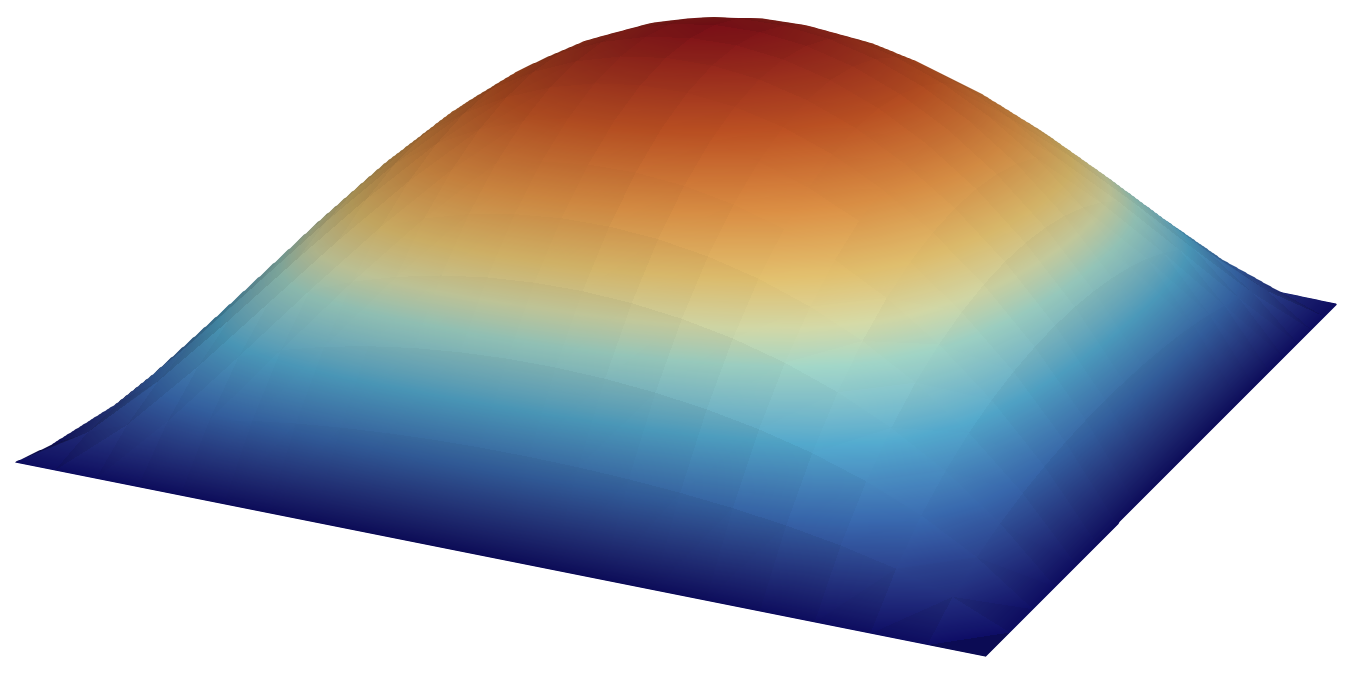
\includegraphics[width=5cm]{images/global-solution.png}};
    \node[inner sep=0] (topRectangle) at (topImg) 
        {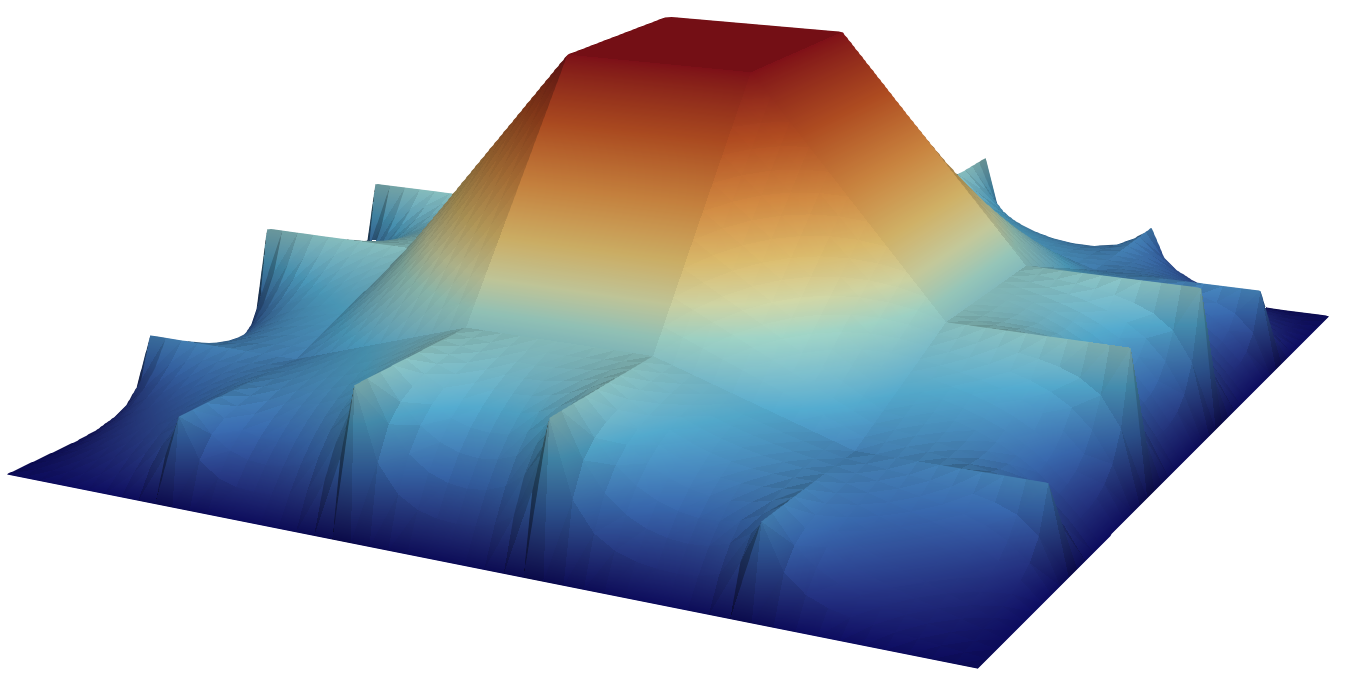
\includegraphics[width=5cm]{images/coarse-solution.png}};
     \node[inner sep=0] (bottomRectangle) at (bottomImg) 
        {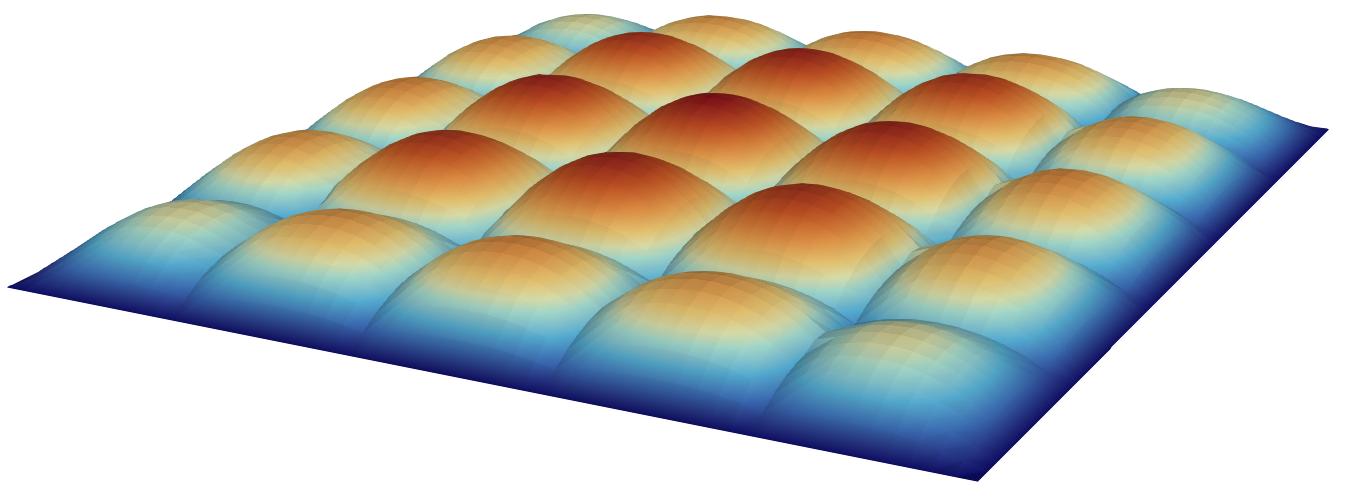
\includegraphics[width=5cm]{images/local-solutions.png}};
    
    \node[fill=white, fill opacity=0.7, text opacity=1, yshift=5mm, xshift=2mm, text width = 35mm] at (leftRectangle.north) {\small Discretized nonlinear problem};
    \node[yshift=0cm, fill=white, fill opacity=0.9, text opacity=1] at (leftRectangle.south) {\small $F(u) = 0$};

    \node[yshift=0cm, fill=white, fill opacity=0.9, text opacity=1] at (bottomRectangle.south) {\small $R_i F\left(\bm{u} - R_i^T T_i(\bm{u})\right) = 0$};
    
    \node [fill=white, fill opacity=0.9, text opacity=1] at (topRectangle.south){\small $\Phi^T F\left(\bm{u} - \Phi T_0(\bm{u})\right) = 0$};
    
    \node[align=left, fill=white, fill opacity=0.7, text opacity=1, text width = 4.5cm] at (9.6,-1.3){\small Solve with Newton's method for nonlinear corrections $T_i(u), \quad i = 0,\ldots, N$};
    
    \node[draw, rectangle, minimum width=4cm, minimum height=1cm] (boxedEq) at (rightEq) {\small $\mathcal{F}(\bm{u}) = \sum_{i=0}^{N} R_i^T T_i(\bm{u})$};
    
    % Arrows
    \draw[-{Stealth[length=3mm, width=2mm]}] ($(leftRectangle.north east) + (-0.5, -0.5)$) -- ($(topRectangle.south west) + (0.3, 0.3)$);
    \draw[-{Stealth[length=3mm, width=2mm]}] ($(leftRectangle.south east) + (-0.7, 0.4)$) -- ($(bottomRectangle.north west) + (0.8, -0.2)$);
    \draw[-{Stealth[length=3mm, width=2mm]}] ($(topRectangle.south east)+ (-0.3, 0.7)$) -- ($(boxedEq.north west)+ (-0.1, 0.1)$);
    \draw[-{Stealth[length=3mm, width=2mm]}] ($(bottomRectangle.north east)+ (-0.8, -0.1)$) -- ($(boxedEq.south west)+ (-0.1, -0.1)$);
\end{tikzpicture}

\end{frame}
